\chapter{Introduzione}

\section{Definizioni}

\begin{definizione}[Gioco]
    Un \textbf{gioco} è una struttura definita da: un insieme di $n$ giocatori $\{1, 2, \dots, n\}$, dove ogni giocatore $i$ possiede un \textit{insieme di strategie} $S_i$. Durante il gioco, ogni giocatore $i$ seleziona una strategia $s_i \in S_i$. Il vettore $s = (s_1, \dots, s_n)$ rappresenta il \textit{profilo di strategie} collettivo.
\end{definizione}

\begin{definizione}[Payoff]
    Ogni combinazione di strategie genera un esito numerico per ciascun giocatore, denominato \textbf{payoff (utilità)}:
    \[
    p_i\ :\ S_1 \times S_2 \times \dots \times S_n \to \mathbb{R}
    \]
    Il payoff quantifica il valore che il giocatore intende massimizzare (se rappresenta un guadagno) o minimizzare (se rappresenta un costo). Crucialmente, il payoff del giocatore $i$ dipende sia dalla propria strategia che dalle strategie degli altri $n-1$ giocatori.
\end{definizione}

\begin{definizione}[Payoff Matrix]
    Poiché il risultato dipende dall'incrocio delle scelte di tutti, il gioco può essere rappresentato come una matrice, detta \textbf{matrix payoff}.
    \begin{itemize}
        \item La dimensione della matrice è data dala prodotto cartesiano degli insiemi delle strategie: $S_1 \times S_2 \times \dots \times S_n$.
        \item Ogni cella della matrice contiene il vettore dei payoff $(p1, p2, \dots, p_n)$ corrispondente a quella specifica combinazione di strategie.
    \end{itemize}
\end{definizione}

Per chiarire, immaginiamo un gioco con 2 giocatori, dove ognuno ha 2 strategie: $S_1 = \{A, B\},\ S_2 = \{C, D\}$. La matrice dei payoff $S_1 \times S_2$ avrà 4 celle, e in ogni cella ci saranno due numeri: il guadagno del giocatore 1 e quello del giocatore 2.

\begin{table}[H]
    \centering
    \renewcommand{\arraystretch}{1.5} % Aumenta lo spazio verticale per leggibilità
    \caption{Rappresentazione in Forma Normale (Matrice dei Payoff)}
    \label{tab:matrice_generica}
    \begin{tabular}{|c|c|c|}
        \hline
        \diagbox{\textbf{G1}}{\textbf{G2}} & \textbf{Strategia $s_{2A}$} & \textbf{Strategia $s_{2B}$} \\
        \hline
        \textbf{Strategia $s_{1A}$} & $(p_1, p_2)$ & $(p_1, p_2)$ \\
        \hline
        \textbf{Strategia $s_{1B}$} & $(p_1, p_2)$ & $(p_1, p_2)$ \\
        \hline
    \end{tabular}
\end{table}

\section{Equilibri}

Avendo definito i concetti fondamentali della teoria dei giochi, l'obiettivo successivo consiste nell'identificare l'esito finale (soluzione) del gioco, considerando il comportamento razionale e egoistico di ogni giocatore. In particolare, si cerca di determinare un \textbf{equilibrio}, ossia uno stato in cui nessun giocatore ha incentivo a deviare dalla propria strategia.

Per definire formalmente l'equilibrio, è utile introdurre una notazione compatta per indicare le strategie di \textit{tutti gli altri} giocatori.
Dato un profilo di strategie $s = (s_1, s_2, \dots, s_n)$, indichiamo con $s_{-i}$ il profilo delle strategie di tutti i giocatori eccetto il giocatore $i$:
\[
s_{-i} = (s_1, \dots, s_{i-1}, s_{i+1}, \dots, s_n)
\]
Di conseguenza, possiamo riscrivere il profilo completo come $s = (s_i, s_{-i})$.

\begin{definizione}[Strategie Dominanti e Equilibrio]
    Una strategia $s_i^* \in S_i$ è detta \textbf{dominante} per il giocatore $i$ se, \textbf{indipendentemente dalle scelte degli altri giocatori}/, garantisce un payoff sempre migliore (o uguale) rispetto a qualsiasi altra strategia disponibile.
    
    Formalmente, $s_i^*$ domina $s_i$ se per ogni profilo di strategie degli altri giocatori $s_{-i} = (s_1, \dots, s_{i-1}, s_{i+1}, \dots, s_n)$:
    \begin{itemize}
        \item Se $p_i$ è un payoff di \textit{guadagno}: $p_i(s_i^*, s_{-i}) \ge p_i(s_i, s_{-i})$
        \item Se $p_i$ è un payoff di \textit{costo}: $p_i(s_i^*, s_{-i}) \le p_i(s_i, s_{-i})$
    \end{itemize}
    
    Un \textbf{Dominant Strategy Equilibrium} è un profilo di strategie $s^* = (s_1^*, s_2^*, \dots, s_n^*)$ dove $s_i^*$ è una strategia dominante per ogni giocatore $i$.
\end{definizione}

\begin{definizione}[Equilibrio di Nash]
    Un profilo di strategie $s^* = (s_1^*, s_2^*, \dots, s_n^*)$ è un \textbf{Equilibrio di Nash} se, per ogni giocatore $i$ e per ogni possibile strategia alternativa $s_i \in S_i$, vale la seguente condizione:
    \[
    p_i(s_i^*, s_{-i}^*) \geq p_i(s_i, s_{-i}^*)
    \]
    In parole semplici, la strategia $s_i^*$ è la \textit{miglior risposta} (best response) alle strategie $s_{-i}^*$ giocate dagli altri. Nessun giocatore ha un incentivo a deviare unilateralmente dalla propria strategia.
\end{definizione}

Sulla base di queste definizioni, possiamo fare due importanti osservazioni pratiche:

\begin{osservazione}[Convergenza immediata]
Se un gioco possiede un DSE, i giocatori razionali convergeranno immediatamente su di esso.
A differenza dell'equilibrio di Nash generale, qui i giocatori non devono fare previsioni o congetture su cosa faranno gli avversari: la scelta ottima è univoca e indipendente dal contesto.
\end{osservazione}

\begin{osservazione}[Rarità del DSE]
Sebbene il DSE sia una soluzione ideale per la sua stabilità e semplicità, è una condizione molto restrittiva. Nella pratica, \textbf{pochissimi giochi} possiedono un equilibrio in strategie dominanti. La maggior parte delle situazioni strategiche richiede di adattare la propria scelta in base alle aspettative sul comportamento altrui (rientrando quindi nel più ampio concetto di Equilibrio di Nash).
\end{osservazione}

\section{Esempi di Giochi}

\begin{description}
    \item[The Prisoner's Dilemma] Due prigionieri sono sotto processo per un crimine e ciascuno deve scegliere se confessare il reato o rimanere in silenzio. Se entrambi rimangono in silenzio, le autorità non saranno in grado di provare le accuse a loro carico e sconteranno entrambi una pena detentiva breve, ad esempio 2 anni, per reati minori. Se invece solo uno dei due confessa, la sua pena sarà ridotta a 1 anno e verrà utilizzato come testimone contro l'altro, il quale riceverà una condanna a 5 anni. Infine, se entrambi confessano, otterranno entrambi un leggero sconto di pena per aver collaborato con le autorità e dovranno scontare 4 anni di carcere ciascuno (invece di 5).
    
    Chiaramente, vi sono quattro esiti possibili a seconda delle scelte effettuate da ciascuno dei due prigionieri. Possiamo riassumere sinteticamente i costi sostenuti in questi quattro scenari attraverso la seguente matrice $2 \times 2$.

    \begin{table}[H]
        \centering
        \renewcommand{\arraystretch}{1.5} % Aumenta lo spazio verticale per leggibilità
        \caption{Rappresentazione in Forma Normale del gioco "The Prisoner's Dilemma"}
        \begin{tabular}{|c|c|c|}
            \hline
            \diagbox{$\mathbf{P_1}$}{$\mathbf{P_2}$} & \textbf{Confessa} & \textbf{Non Confessa} \\
            \hline
            \textbf{Confessa} & $(4, 4)$ & $(1, 5)$ \\
            \hline
            \textbf{Non Confessa} & $(5, 1)$ & $(2, 2)$ \\
            \hline
        \end{tabular}
        \label{tab:The Prisoner's Dilemma}
    \end{table}

    Dalla matrice dei costi emerge che confessare è la strategia dominante per entrambi i giocatori, indipendentemente dalla scelta dell'avversario. Di conseguenza, il profilo \texttt{(Confessa, Confessa)} costituisce un \textbf{DSE}. È interessante notare che, sebbene \texttt{(Non Confessa, Non Confessa)} comporti pene minori per entrambi, ogni giocatore ha incentivo a deviare unilateralmente e confessare per ridurre la propria pena a 1 anno. Pertanto, \texttt{(Non Confessa, Non Confessa)} non è un equilibrio.
    
    \item[ISP Routing Game] Consideriamo due ISP che devono instradare traffico attraverso punti di peering (\autoref{fig:isp_routing}). Ogni ISP sceglie il percorso minimizzando i propri costi, ignorando l'impatto sugli altri. 

        \begin{figure}[ht!]
            \centering
            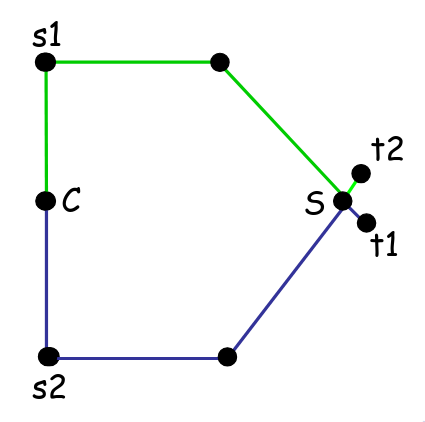
\includegraphics[width=0.35\textwidth]{images/isp_game.png}
            \caption{ISP Routing Network Topology}
            \label{fig:isp_routing}
        \end{figure}

    \begin{description}
        \item[\textcolor{green}{ISP1}] deve inviare traffico dal nodo sorgente $s_1$ al nodo destinazione $t_1$ e controlla gli archi verdi.
        \item[\textcolor{blue}{ISP2}] deve inviare traffico dal nodo sorgente $s_2$ al nodo destinazione $t_2$ e controlla gli archi blu.
    \end{description}
    \textbf{Strategie:} Esistono due punti di peering attraverso cui instradare il traffico: il punto $C$ e il punto $S$. Pertanto, lo spazio delle strategie per entrambi è 
    \[
        S_i = \{\text{Through } S, \text{Through } C\}.
    \]
    \textbf{Costi:} I link lunghi hanno un costo unitario di 1 per il proprietario del link. Questo significa che il costo del link viene pagato dal proprietario e non da chi sta inviando traffico su quel link. Infatti, $s_1$ può decidere se passare per $S$ pagando 2, oppure passar per $C$ e pagare solo 1, analogamente per $s_2$.

    \begin{table}[H]
        \centering
        \renewcommand{\arraystretch}{1.5} % Aumenta lo spazio verticale per leggibilità
        \caption{Matrice dei Costi del Network Game}
        \begin{tabular}{|c|c|c|}
            \hline
            \diagbox{\textbf{ISP1}}{\textbf{ISP1}} & \textbf{Through $S$}  & \textbf{Through $C$} \\
            \hline
            \textbf{Through $S$} & $(2, 2)$ & $(5, 1)$ \\
            \hline
            \textbf{Through $C$} & $(1, 5)$ & $(4, 4)$ \\
            \hline
        \end{tabular}
        \label{tab:ISP Routing Game}
    \end{table}

    L'unico Equilibrio di Nash (in strategie dominanti) è la coppia $(C, C)$, con un costo di $(4, 4)$.
    Tuttavia, notiamo che la configurazione $(S, S)$ avrebbe garantito un costo molto inferiore $(2, 2)$ per entrambi. Questo è un classico esempio di \textbf{Dilemma del Prigioniero}: la razionalità individuale porta a un risultato socialmente inefficiente.
    
    \item[The Battle of the Sexes] Esaminiamo ora un gioco di natura completamente diversa: il cosiddetto \textbf{Gioco di Coordinamento}. A differenza dei dilemmi precedenti, in questo scenario i giocatori traggono beneficio principalmente dall'essere nello stesso posto, anche se hanno preferenze diverse su quale luogo scegliere. 
        
    L'esempio classico presenta due persone (tradizionalmente indicate come "Uomo" e "Donna") che desiderano passare la serata insieme, ma con preferenze divergenti su dove andare. Entrambi hanno a disposizione due opzioni: andare allo \textbf{Stadio} oppure andare al \textbf{Cinema}. L'Uomo preferisce lo Stadio e riceve maggiore soddisfazione dal trascorrere la serata lì, mentre la Donna preferisce il Cinema. Tuttavia, entrambi preferiscono decisamente stare insieme piuttosto che andare da soli nel luogo che ciascuno preferisce. Questo gioco illustra come la coordinazione sia spesso più importante della realizzazione delle preferenze individuali.

    I numeri rappresentano il livello di soddisfazione (utilità). Notiamo che i valori sono alti quando le scelte coincidono (diagonale principale) e bassi quando divergono.
    
    \begin{table}[H]
        \centering
        \renewcommand{\arraystretch}{1.5} % Aumenta lo spazio verticale per leggibilità
        \caption{Matrice del gioco The Battle of the Sexes}
        \begin{tabular}{|c|c|c|}
            \hline
            \diagbox{\textbf{Uomo}}{\textbf{Donna}} & \textbf{Stadio}  & \textbf{Cinema} \\
            \hline
            \textbf{Stadio} & $(6, 5)$ & $(2, 2)$ \\
            \hline
            \textbf{Cinema} & $(1, 1)$ & $(5, 6)$ \\
            \hline
        \end{tabular}
        \label{tab:The Battle of the Sexes}
    \end{table}
    Analizzando la matrice, emergono due differenze fondamentali rispetto al Dilemma del Prigioniero: non esiste una strategia che sia \textit{sempre} la migliore.
    \begin{itemize}
        \item Se la Donna va allo Stadio, all'Uomo conviene andare allo Stadio ($6 > 1$).
        \item Se la Donna va al Cinema, all'Uomo conviene andare al Cinema ($5 > 2$).
    \end{itemize}
    La scelta ottima dipende strettamente dalla scelta dell'altro. Infatti come possiamo osservare, non ci sono DSE.

    Esistono due Equilibri di Nash puri:
    \begin{itemize}
        \item \textbf{(Stadio, Stadio):} Payoff $(6, 5)$. Nessuno ha incentivo a deviare (l'Uomo perderebbe utilità passando da 6 a 1, la Donna da 5 a 2).
        \item \textbf{(Cinema, Cinema):} Payoff $(5, 6)$. Analogamente, nessuno ha incentivo a cambiare strategia da solo.
    \end{itemize}
\end{description}

\section{Esistena di un NE}

Dopo aver analizzato diverse tipologie di giochi, è fondamentale discutere le proprietà teoriche generali dell'Equilibrio di Nash (NE), in particolare riguardo la sua esistenza e la relazione con le strategie dominanti.

Un problema centrale nella Teoria dei Giochi riguarda la garanzia che un equilibrio esista sempre.
Purtroppo, limitandosi alle sole \textbf{strategie pure} (come quelle viste finora: confessare/non confessare, stadio/cinema), non esiste un risultato generale di esistenza.

A seconda del gioco, possiamo trovarci di fronte a tre scenari:
\begin{enumerate}
    \item \textbf{Nessun Equilibrio (No NE):} Il gioco non possiede alcun punto stabile in strategie pure (es. Sasso-Carta-Forbice giocato in modo deterministico).
    \item \textbf{Unico Equilibrio (One NE):} Esiste una sola soluzione stabile (es. Dilemma del Prigioniero).
    \item \textbf{Molteplici Equilibri (Many NE):} Esistono più soluzioni stabili e sorge il problema del coordinamento (es. Battaglia dei Sessi).
\end{enumerate}

Esiste una precisa gerarchia logica tra l'Equilibrio in Strategie Dominanti (DSE) e l'Equilibrio di Nash. Poiché in un NE nessun agente può deviare unilateralmente con profitto, e una strategia dominante è ottima contro \textit{tutto} (inclusa la strategia di equilibrio dell'altro), vale la seguente implicazione:

\[
\textbf{Dominant Strategy Equilibrium (DSE)} \implies \textbf{Nash Equilibrium (NE)}
\]

\begin{osservazione}
\textbf{Il viceversa non è vero.} Un Equilibrio di Nash non è necessariamente un equilibrio in strategie dominanti. Nella "Battaglia dei Sessi", ad esempio, gli esiti (Stadio, Stadio) sono NE ma non DSE.
\end{osservazione}

Le definizioni viste assumono che i giocatori "deliberino" sulle strategie degli altri in un singolo incontro (One-shot game). Tuttavia, se il gioco viene giocato \textbf{ripetutamente} nel tempo:
Se i giocatori convergono verso una soluzione stabile in cui nessuno cambia più la propria scelta, allora quella soluzione \textbf{deve essere necessariamente} un Equilibrio di Nash.

Come abbiamo visto, limitandosi alle strategie pure non è garantita l'esistenza di un equilibrio. Tuttavia, lo scenario cambia radicalmente se estendiamo le possibilità d'azione dei giocatori introducendo la casualità.

\begin{definizione}[Strategia Mista]
    Una \textbf{strategia mista} consiste nel selezionare la propria azione in modo casuale, utilizzando una \textbf{distribuzione di probabilità} sull'insieme delle strategie possibili.
    Invece di scegliere deterministicamente "A" o "B", il giocatore sceglie di giocare "A" con probabilità $p$ e "B" con probabilità $1-p$.
    In questo contesto, l'obiettivo del giocatore razionale diventa la massimizzazione del \textbf{payoff atteso} (expected payoff).
\end{definizione}
    

John Nash ha dimostrato un risultato fondamentale che garantisce l'esistenza della soluzione per una vastissima classe di giochi.

\begin{teorema}[Teorema di Nash, 1951]\label{th:nash}
Ogni gioco con un numero \textbf{finito} di giocatori e un numero \textbf{finito} di strategie ammette \textbf{almeno un Equilibrio di Nash in strategie miste}.
\end{teorema}

In un equilibrio a strategie miste, nessun giocatore può migliorare il proprio payoff atteso modificando unilateralmente la propria distribuzione di probabilità.

\subsection{Esempio: Matching Pennies}
Un caso fondamentale è rappresentato dai giochi puramente conflittuali (a somma zero), come il "Matching Pennies" (Testa o Croce). In questo scenario, gli interessi dei giocatori sono diametralmente opposti.

Due giocatori mostrano contemporaneamente una moneta.
\begin{itemize}
    \item \textbf{Giocatore I (P1):} Vince se le monete sono uguali (Testa-Testa o Croce-Croce).
    \item \textbf{Giocatore II (P2):} Vince se le monete sono diverse (Testa-Croce o Croce-Testa).
\end{itemize}

I payoff sono $(1, -1)$ se vince P1 e $(-1, 1)$ se vince P2. La somma è sempre 0.

\begin{table}[H]
    \centering
    \renewcommand{\arraystretch}{1.5} % Aumenta lo spazio verticale per leggibilità
    \caption{Matrice del gioco Matching Pennies}
    \begin{tabular}{|c|c|c|}
        \hline
        \diagbox{\textbf{P1}}{\textbf{P2}} & \textbf{Testa}  & \textbf{Croce} \\
        \hline
        \textbf{Testa} & $(1, -1)$ & $(-1, 1)$ \\
        \hline
        \textbf{Croce} & $(-1, 1)$ & $(1, -1)$ \\
        \hline
    \end{tabular}
    \label{tab:Matching Pennies}
\end{table}

In qualsiasi configurazione ci troviamo, uno dei due giocatori preferirà sempre cambiare la propria strategia per migliorare il proprio payoff. Di conseguenza, \textbf{non esiste alcun Equilibrio di Nash in strategie pure}.

Se invece applichiamo il \autoref{th:nash}, la situazione cambia drasticamente. Consideriamo il caso in cui ogni giocatore adotta una strategia mista in cui sceglie \textbf{Testa} e \textbf{Croce} con uguale probabilità:
\[
p(\text{Testa}) = p(\text{Croce}) = 0.5
\]

In questa configurazione, il payoff atteso per entrambi i giocatori risulta essere esattamente 0. Ciò che rende questa soluzione particolarmente interessante è che costituisce un \textbf{Equilibrio di Nash}: dato che l'avversario sta giocando in modo casuale con probabilità 50/50, non esiste alcuna strategia alternativa, che sia pura o mista, capace di fornirmi un vantaggio superiore a 0. Se io dovessi deviare dalla strategia 50/50, cambiando ad esempio a giocare sempre Testa, l'avversario potrebbe sfruttare questa prevedibilità per contrastarmi. Di conseguenza, il payoff atteso non migliora affatto rispetto alla situazione di equilibrio, e nessun giocatore ha incentivo a deviare dalla strategia mista 50/50.

\section{Come Analizzare un Gioco}

Quando si modella una situazione reale attraverso la Teoria dei Giochi (ad esempio, il routing in una rete), l'analisi non si limita a definire la matrice dei payoff. Esistono quattro problemi tipici che devono essere affrontati sistematicamente:

\begin{description}
    \item[Esistenza (Existence):]
    Il primo passo è stabilire se il gioco ammette sempre un Equilibrio di Nash (NE).
    \begin{itemize}
        \item In strategie pure? Non sempre (come visto in Matching Pennies).
        \item In strategie miste? Sì, garantito dal Teorema di Nash (per giochi finiti).
    \end{itemize}

    \item[Individuazione (Finding a NE):]
    Una volta stabilito che un equilibrio esiste, il problema diventa algoritmico: come facciamo a trovarlo?
    \begin{itemize}
        \item È facile da calcolare?
        \item Richiede algoritmi complessi?
    \end{itemize}

    \item[Convergenza (Convergence):]
    Nei contesti di rete, i giochi spesso non sono statici (One-shot) ma ripetuti nel tempo. La domanda cruciale è: il sistema dinamico convergerà eventualmente verso un equilibrio?
    \begin{itemize}
        \item Se sì, in \textbf{quanti passi}? La velocità di convergenza è fondamentale per le applicazioni reali (es. protocolli internet).
    \end{itemize}

    \item[Qualità (Quality of NE):]
    Il fatto che un equilibrio esista ed sia stabile non significa che sia "buono".
    \begin{itemize}
        \item L'equilibrio è efficiente per la società (come nel coordinamento perfetto) o disastroso (come nel Dilemma del Prigioniero)?
        \item In Analisi di Reti, questo punto introduce il concetto di \textit{Price of Anarchy} (PoA): quanto perdiamo in efficienza a causa dell'egoismo dei singoli rispetto a una soluzione centralizzata ottima?
    \end{itemize}
\end{description}

Una volta stabilito che un equilibrio esiste e sappiamo come trovarlo, sorge una domanda fondamentale sulla sua \textbf{efficienza}.
Spesso, l'esito derivante dalle scelte egoistiche dei singoli (NE) è molto diverso dall'esito "ideale" che si otterrebbe se i giocatori collaborassero per il bene comune.

Per quantificare questa inefficienza, dobbiamo prima definire cosa intendiamo per "risultato migliore".

\begin{definizione}[Funzione di Scelta Sociale]
Sia $S = S_1 \times \dots \times S_n$ l'insieme di tutti i possibili profili di strategia. Una \textbf{Funzione di Scelta Sociale} (o funzione di costo sociale) è una funzione:
\[
C: S \to \mathbb{R}
\]
che misura la qualità complessiva di un determinato esito $s \in S$.
\end{definizione}

La forma più comune di questa funzione è la somma dei risultati individuali (approccio utilitaristico):

\begin{itemize}
    \item \textbf{Minimizzazione dei Costi (Social Cost):}
    Nei giochi di rete (es. routing), solitamente si vuole minimizzare la somma dei ritardi o dei costi di tutti gli utenti:
    \[
    C(s) = \sum_{i=1}^{N} \text{cost}_i(s)
    \]
    In questo caso, l'ottimo sociale è il profilo $s^*$ che \textit{minimizza} $C(s)$.

    \item \textbf{Massimizzazione dell'Utilità (Social Welfare):}
    Nei giochi economici, si vuole massimizzare la somma dei profitti:
    \[
    SW(s) = \sum_{i=1}^{N} \text{utility}_i(s)
    \]
    In questo caso, l'ottimo sociale è il profilo che \textit{massimizza} la somma.
\end{itemize}

\newpage

\subsection{Price of Anarchy (PoA)}

Definita la funzione di scelta sociale, possiamo ora definire il "prezzo dell'anarchia", ossia:

\begin{definizione}[Price of Anarchy]
    Sia $G$ un gioco con insieme di Equilibri di Nash $S$, e sia $C$ una funzione di scelta sociale. Denotiamo con $OPT$ il profilo di strategie che ottimizza globalmente $C$.
    
    Il \textbf{Price of Anarchy} (PoA) misura il rapporto tra la qualità del peggior equilibrio di Nash e la qualità della soluzione ottima:
    \begin{itemize}
        \item Se $C$ rappresenta un \textit{costo} (da minimizzare):
        \[
        PoA_G(C) = \max_{s \in S} \frac{C(s)}{C(OPT)}
        \]
        \item Se $C$ rappresenta un'\textit{utilità} (da massimizzare):
        \[
        PoA_G(C) = \min_{s \in S} \frac{C(s)}{C(OPT)}
        \]
    \end{itemize}
    
    Un valore $PoA = 1$ indica che il peggior equilibrio raggiunge l'ottimo; valori superiori a 1 quantificano l'inefficienza causata dall'egoismo dei giocatori.
\end{definizione}

\subsection{Price of Stability (PoS)}

Mentre il Price of Anarchy misura il peggior caso, il \textbf{Price of Stability} si concentra sul migliore equilibrio raggiungibile.

\begin{definizione}[Price of Stability]
    Sia $G$ un gioco con insieme di Equilibri di Nash $S$, e sia $C$ una funzione di scelta sociale. Denotiamo con $OPT$ il profilo di strategie che ottimizza globalmente $C$.
    
    Il \textbf{Price of Stability} (PoS) misura il rapporto tra la qualità del migliore equilibrio di Nash e la qualità della soluzione ottima:
    \begin{itemize}
        \item Se $C$ rappresenta un \textit{costo} (da minimizzare):
        \[
        PoS_G(C) = \min_{s \in S} \frac{C(s)}{C(OPT)}
        \]
        \item Se $C$ rappresenta un'\textit{utilità} (da massimizzare):
        \[
        PoS_G(C) = \max_{s \in S} \frac{C(s)}{C(OPT)}
        \]
    \end{itemize}
    
    Un valore $PoS = 1$ indica che il migliore equilibrio coincide con l'ottimo; valori superiori a 1 quantificano quanto il miglior equilibrio rimane lontano dall'ottimale.
\end{definizione}

\subsubsection{Proprietà di PoA e PoS}

\begin{description}
    \item[Range di Valori] 
    Il valore ideale è sempre 1. Per problemi di minimizzazione: $1 \le \text{PoS} \le \text{PoA}$. Per problemi di massimizzazione: $\text{PoA} \le \text{PoS} \le 1$.
    
    \item[Relazione tra PoA e PoS]
    Poiché PoA misura il peggior equilibrio e PoS il migliore, vale sempre $\text{PoS} \le \text{PoA}$ (in valore assoluto). Se esiste un \textbf{unico equilibrio}, allora $\text{PoA} = \text{PoS}$.
    
    \item[Interpretazione] I valori di PoA e PoS possono essere interpretati nel seguente modo:
    \begin{itemize}
        \item \textbf{PoA (worst-case):} Garantisce che il sistema non degraderà oltre un certo limite.
        \item \textbf{PoS (best-case):} Assicura che esista almeno una soluzione stabile buona, anche se non è detto che la raggiungeremo.
    \end{itemize}
    
    \item[Quando usare PoS?]
    Il PoA spesso è troppo elevato. Il PoS invece quantifica la minima degradazione dovuta al solo vincolo di stabilità, permettendo di valutare se un buon risultato è almeno possibile.
\end{description}

\subsection{Selfish Routing e l'Esempio di Pigou}

Dopo aver introdotto le metriche di efficienza (PoA), applichiamo questi concetti a uno scenario reale fondamentale per le reti di telecomunicazione: il \textbf{Selfish Routing}.

Possiamo modellare una grande rete di traffico (come Internet o il traffico stradale) utilizzando la Teoria dei Giochi, facendo alcune assunzioni specifiche per gestire l'elevato numero di utenti:

\begin{itemize}
    \item \textbf{Giocatori e Strategie:} Sono gli utenti della rete che scelgono i percorsi (paths) su cui instradare il proprio traffico.
    \item \textbf{Natura "Non-atomica":} Esiste un numero molto grande di utenti, ognuno controllando una frazione infinitesimale del traffico totale e incapace di influenzare la congestione globale.
    \item \textbf{Funzioni di Costo e Obiettivo:} Ogni arco ha una funzione di latenza basata sulla congestione; ogni utente minimizza il proprio tempo di percorrenza (egoisticamente), mentre l'obiettivo globale è minimizzare il tempo medio di percorrenza di tutti gli utenti.
\end{itemize}

\newpage

\subsubsection{Il Gioco di Pigou (1920)}
Consideriamo una rete semplice con un punto di partenza $s$ e un punto di arrivo $t$, collegati da due strade parallele, su cui deve transitare \textbf{1 unità di traffico} totale.

\begin{figure}[ht!]
    \centering
    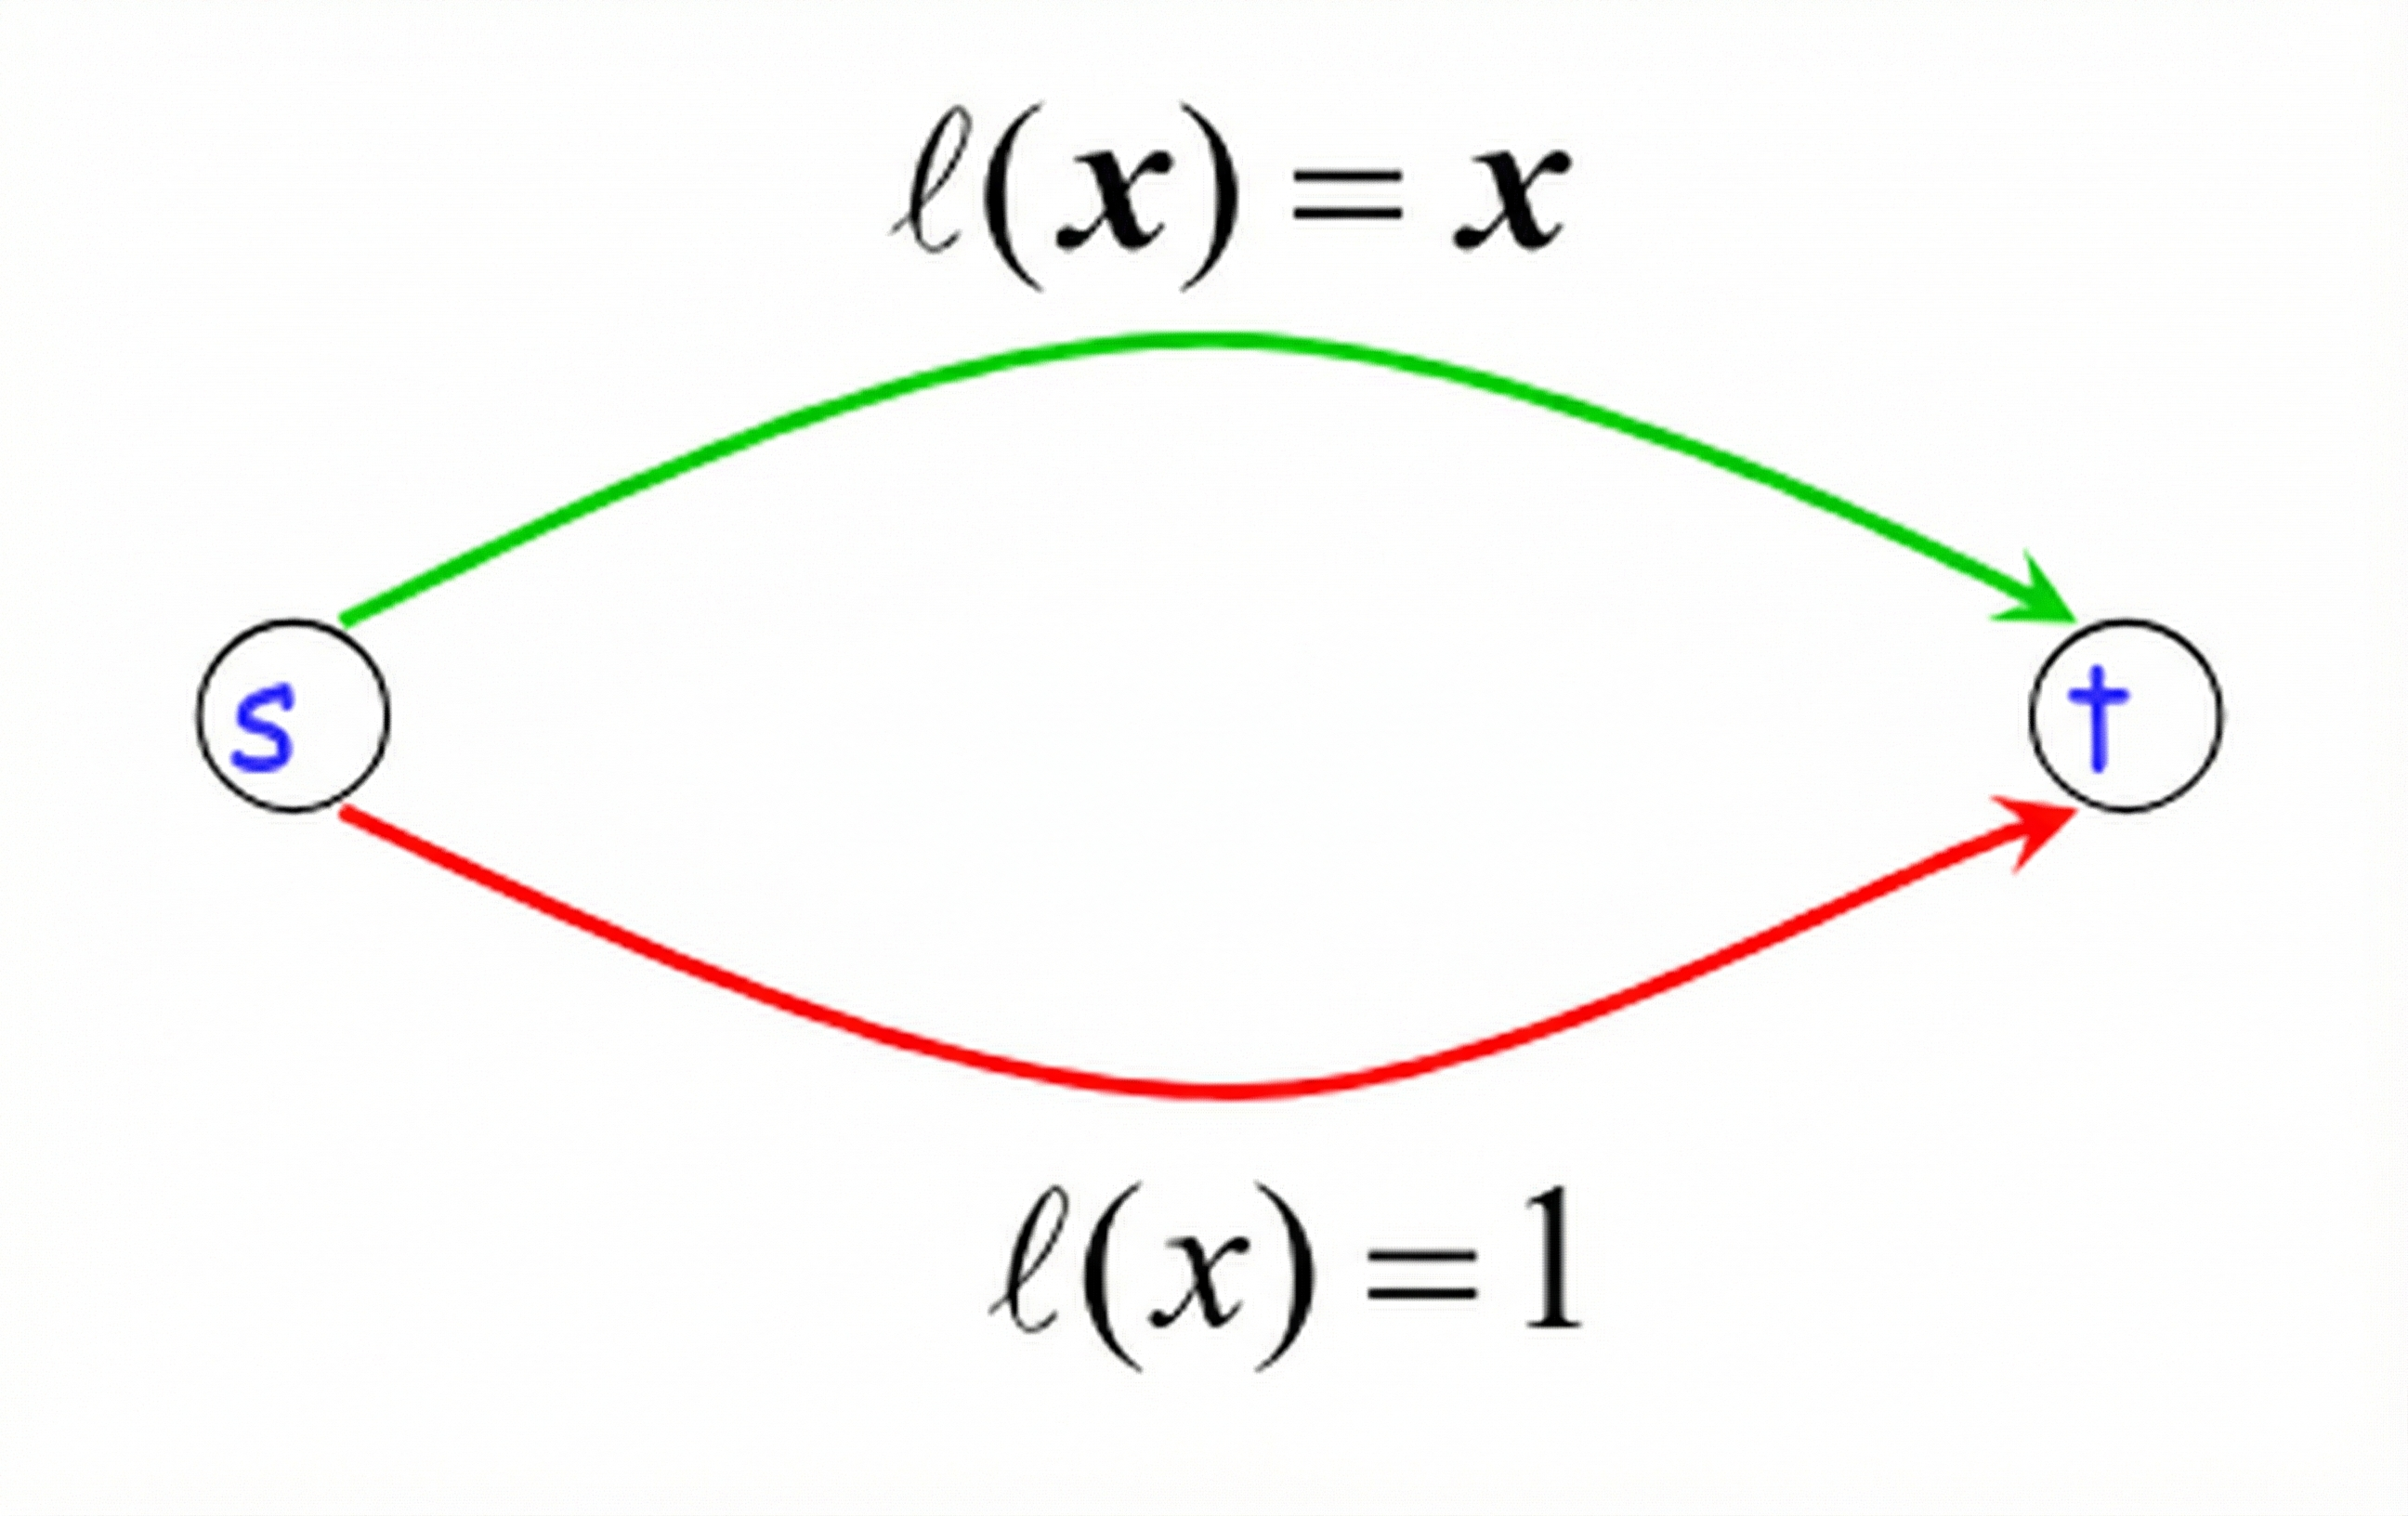
\includegraphics[width=0.4\textwidth]{images/selfish.png}
\end{figure}

Analizziamo la differenza tra l'equilibrio egoistico e l'ottimo sociale.

Ogni utente sceglie la strada più veloce.
\begin{itemize}
    \item Se un utente sceglie la strada superiore, paga $x$ (dove $x$ è la frazione di flusso su quella strada).
    \item Poiché il flusso totale è 1, il valore massimo di $x$ è 1.
    \item Dato che il costo della strada inferiore è fisso a 1, e la strada superiore costa al massimo 1 (quando è piena), agli utenti converrà sempre riempire la strada superiore fino al limite.
\end{itemize}
\textbf{Risultato NE:} Tutto il flusso ($x=1$) passa sopra.
\[
\text{Costo Sociale (NE)} = 1 \cdot 1 + 0 \cdot 1 = 1
\]
Tutti pagano 1.

Un pianificatore centrale può dividere il traffico per minimizzare il costo totale $C(x)$.
Se inviamo una frazione $x$ sopra e $(1-x)$ sotto, il costo totale è:
\[
C(x) = x \cdot \ell_{top}(x) + (1-x) \cdot \ell_{bot}(1-x) = x \cdot x + (1-x) \cdot 1 = x^2 + 1 - x
\]
Per trovare il minimo, calcoliamo la derivata e poniamola a 0:
\[
\frac{d}{dx}(x^2 - x + 1) = 2x - 1 = 0 \implies x_{OPT} = \frac{1}{2}
\]
L'ottimo si ottiene dividendo il traffico a metà ($0.5$ sopra, $0.5$ sotto).
\[
\text{Costo Sociale ($x_{OPT}$)} = \frac{1}{2} \cdot \frac{1}{2} + \frac{1}{2} \cdot 1 = 0.25 + 0.5 = 0.75
\]

Confrontando i due costi otteniamo il PoA per questo scenario:
\[
\text{PoA} = \frac{\text{Costo NE}}{\text{Costo OPT}} = \frac{1}{0.75} = \frac{4}{3} \approx 1.33
\]
\begin{osservazione}
Questo risultato ($4/3$) è celebre perché rappresenta il \textbf{massimo Price of Anarchy possibile} per reti con funzioni di latenza lineari (affini). Significa che, in questo tipo di reti, l'anarchia non aumenta i costi più del 33\% rispetto alla gestione centralizzata.
\end{osservazione}
